\documentclass[10pt]{article}

\usepackage{tmlr}

\usepackage[utf8]{inputenc}
\usepackage[T1]{fontenc}
\usepackage{url}
\usepackage{booktabs}
\usepackage{longtable}
\usepackage{amsfonts}
\usepackage{nicefrac}
\usepackage{microtype}
\PassOptionsToPackage{table}{xcolor}
\usepackage{xcolor}
\definecolor{linkblue}{RGB}{0,0,120}
\usepackage{graphicx}
\usepackage{array}
\usepackage{tabularx}
\usepackage{enumitem}
\usepackage{tikz}
\usetikzlibrary{arrows.meta,positioning,shapes.geometric,fit,backgrounds}
\usepackage{placeins}
\usepackage{float}
\usepackage{hyperref}
\hypersetup{
  colorlinks=true,
  citecolor=linkblue,
  linkcolor=linkblue,
  urlcolor=linkblue,
  anchorcolor=linkblue,
  breaklinks=true
}

\title{Designing Benchmarks for Knowledge Work\thanks{Large language models were used as assistive tools for language editing and for the screening, summarization, and classification steps explicitly reported in the manuscript. The authors are responsible for the study design, analysis, results, and final manuscript.}}
\author{Anonymous authors}

\def\month{MM}
\def\year{YYYY}
\def\openreview{\url{https://openreview.net/forum?id=XXXX}}

\begin{document}

\maketitle

\begin{abstract}
AI agents are moving quickly from answering isolated questions toward completing work through tools, software environments, and multi-step workflows. Much of what these systems are now asked to do is knowledge work, where information and expertise are interpreted, produced, and communicated as part of completing work. Benchmarks for this setting are usually described only by their tasks, environments, and metrics, leaving four questions implicit: what part of the work is represented, under what conditions it is tested, what work product the system is expected to leave, and what part of that product the benchmark actually evaluates. We introduce a work-centered benchmark representation with four fields: represented activity, tested setting, required work product, and evaluated result. The representation makes these choices explicit and comparable across benchmark designs. To support activity-level reporting across occupations, we derive an aim-dependent inventory of 18 work activities from O{*}NET task statements and report evidence on semantic coherence, algorithm sensitivity, external ontology legibility in ESCO, and human interpretability. We apply the representation to \textsc{GDPval}, \textsc{OfficeQA Pro}, and \textsc{APEX-SWE}. The case analyses illustrate how occupational deliverables, grounded answers, and executable state changes capture different parts of work within the same representation.
\end{abstract}

\section{Introduction}

AI agents are increasingly asked to complete work beyond isolated questions. Recent systems use external tools, interact with software environments, and complete multi-step workflows across work-facing settings \citep{wang2024survey}.
Much of the work these systems are being designed to perform is knowledge work: labor in which knowledge serves as both the source material and the output of work \citep{drucker1999productivity,davenport2005thinking}.
Knowledge work covers a large share of the labor market \citep{porat1977information}, including many occupations whose tasks center on information processing, judgment, communication, documentation, and coordination, as reflected in O{*}NET task statements \citep{onet2024tasks}.
Because much computer-based work falls within this category, LLM systems are increasingly studied in relation to work-facing tasks \citep{eloundou2023gpts,brynjolfsson2023genai}.

Standard natural language processing (NLP) benchmarks often evaluate bounded input-output behaviors, while work-facing agent benchmarks increasingly add tools, environments, and longer workflows.
Agentic execution and evaluated result are separate design choices. A complex agent task can still be evaluated through a short answer \citep{browsecomp2024}; other benchmarks evaluate artifacts or persistent state changes \citep{kottamasu2026apex}.
These evaluation designs support different interpretations of benchmark success.
A benchmark used to support a work claim therefore needs to connect the work being represented, the setting in which it is performed, the product the work should leave, and the result the benchmark actually evaluates \citep{jacobs2021measurement,kane2013validating}.

Visible content alone does not identify the role, materials, setting, or receiving workflow in which a knowledge-work output was produced.
The same visible output can therefore support different interpretations across work settings.
The final output alone provides limited evidence about downstream coordination and continuation \citep{carlile2004transferring}, including whether it can be checked, revised, filed, executed, or used in a later workflow step.

Benchmark builders already choose tasks, environments, outputs, and scoring rules. Our contribution is a work-centered representation that connects four choices: what activity is represented, under what tested setting, what product the work requires, and what result the benchmark evaluates. The representation can be used prospectively when designing a benchmark or retrospectively to describe what an existing benchmark actually tests; the same record also supports horizontal comparison across benchmarks with different task formats and evaluation targets.
Section~\ref{sec:knowledge-work} explains why work activity, tested setting, and downstream use matter for benchmark design.
Section~\ref{sec:guidelines} defines the representation and its four fields.
It also derives an O{*}NET-based inventory for identifying work activities \citep{onet2024tasks}.
Section~\ref{sec:whybench} demonstrates the approach through three benchmark case analyses: \textsc{GDPval}, \textsc{OfficeQA Pro}, and \textsc{APEX-SWE}.
Section~\ref{sec:altviews} discusses limitations, alternative interpretations, and future directions.
Table~\ref{tab:terms} gives the definitions used throughout the paper.

\begin{table}[!ht]
\caption{Definitions used in this paper.}
\label{tab:terms}
\centering
\footnotesize
\setlength{\tabcolsep}{2pt}
\setlength{\extrarowheight}{1pt}
\renewcommand{\arraystretch}{1.1}
\begin{tabularx}{\linewidth}{@{}>{\raggedright\arraybackslash}p{0.15\linewidth}>{\raggedright\arraybackslash}X@{}}
\toprule
\textbf{Term} & \textbf{Definition} \\
\midrule
Knowledge work &
A form of labor in which knowledge is both the source material and the output \citep{drucker1999productivity,davenport2005thinking}. \\
Work activity &
A recurrent unit of work that can appear across occupations \citep{onet2026overview,abbott1988system}. \\
Benchmark task &
The benchmark-defined task assigned to a system, including its inputs, available actions, environment, and expected submission \citep{bean2025measuring,liang2023helm}. \\
Tested setting &
The benchmark-defined conditions under which the work activity is evaluated, including materials, tools, role, and workflow state \citep{suchman1987plans,hutchins1995cognition}. \\
Work output &
The visible content produced by the system within the task \citep{carlile2002pragmatic}. \\
Work product &
The object left for review, filing, execution, or downstream continuation, including any state or provenance needed for that use \citep{star1989institutional,carlile2004transferring}. \\
Evaluated result &
The part of the submitted output, artifact, or resulting state that the benchmark checks through its metric, tests, or rubric \citep{bean2025measuring,kane2013validating}. \\
\bottomrule
\end{tabularx}
\end{table}

\section{What Knowledge Work Requires}
\label{sec:knowledge-work}

Knowledge work is commonly defined as labor in which knowledge is a primary input and output of work \citep{drucker1999productivity,davenport2005thinking}.
For benchmark design, a bounded task can represent only part of a work activity, setting, or product.
The four fields connect these choices so that the intended work claim and the evidence provided by the benchmark can be read at the same level. Professional work is organized through roles, authority, problem areas, and boundaries of responsibility \citep{abbott1988system}. Freidson similarly describes professionalism as specialized work organized around occupational control and responsibility \citep{freidson2001professionalism}. Similar visible outputs can carry different responsibilities depending on whether they function as advice, analysis, documentation, review, or decision support.

Performance is situated in the conditions in which action occurs. Situated-action theory describes action as organized through local materials, tools, instructions, and social circumstances \citep{suchman1987plans}. Distributed-cognition accounts similarly treat cognition as distributed across people, artifacts, and environments \citep{hutchins1995cognition}. The same work activity can therefore be instantiated differently depending on the materials provided, tools available, role assigned, and workflow constraints imposed by the benchmark.

Knowledge-work outputs also move across actors, systems, and dependent activities. Boundary-object work explains how artifacts support coordination across communities while remaining usable in different local contexts \citep{star1989institutional}. Carlile's work on knowledge boundaries shows that knowledge crossing organizational boundaries often requires representation, translation, and transformation \citep{carlile2002pragmatic,carlile2004transferring}. Coordination theory treats work as the management of dependencies among activities \citep{malone1994coordination}. These perspectives direct attention to the object left for review, filing, execution, or continuation.

For a work-facing benchmark, four choices are separate. Represented activity names the work being evaluated. Tested setting records the conditions under which it occurs. Required work product records what must remain usable for review or continuation. Evaluated result records which parts of that product are checked. A locally correct answer can still be incomplete when the receiving workflow requires more than the benchmark evaluates. The representation concerns benchmark scope and the relation between a work claim and the evidence collected. Sampling, grader reliability, robustness, and fairness are separate benchmark-design questions.

The representation operates at the individual benchmark level. Bean et al. analyze links among phenomenon, task, metric, and claim across LLM benchmarks \citep{bean2025measuring}. In that chain, the task is one link between the phenomenon and the metric. A work-facing task specification also fixes the materials available, the role assigned, the workflow state, and the product expected at completion. Those choices can change the work represented even when two benchmark variants share a task label or metric family. We therefore separate tested setting from required work product, then record which part of that product enters evaluation. Figure~\ref{fig:officeqa-claim} shows the distinction using the same question and source corpus under two work-product requirements.

Wang et al. map agent benchmarks to occupational domains, skills, realism, and autonomy at portfolio scale \citep{wang2026realwork}. That analysis describes where evaluation effort is concentrated across benchmarks. The representation here describes what one benchmark episode represents and evaluates. Portfolio mapping can show which occupations or skills receive coverage; the four fields show what evidence an individual benchmark contributes to that coverage.

\section{A Work-Centered Representation for Benchmark Design and Reporting}
\label{sec:guidelines}
The representation has four parts: (1) represented activity, (2) tested setting, (3) required work product, and (4) evaluated result. These fields describe the work a benchmark represents and the evidence it collects.

\subsection{Represented work activity}
\label{sec:define-work}

Represented activity identifies the work the benchmark is meant to represent. For a work-facing benchmark, the activity is the target construct; a benchmark task is one operationalization of that activity in a particular setting, and one episode may combine several activities. This paper uses \textit{work activity} as a reporting unit between a component capability and an occupation or domain. A component task names a smaller capability, while a domain contains many activities with different roles, materials, products, and downstream uses. A work-activity label names the work while the benchmark report specifies how the task, tested setting, and work product instantiate it.

Current benchmark labels often describe one of three levels. Domain or occupation labels locate a benchmark in an application area, but each label spans activities with different roles, materials, products, and standards of adequacy \citep{handel2016onet,onet2024tasks}. A benchmark can therefore sample a limited part of an occupation while retaining the occupation label. Component labels isolate a smaller behavior \citep{rajpurkar2016squad,nallapati2016cnndm,thakur2021beir}. Retrieval, summarization, and classification can each occur inside a broader activity. Performance on the component alone does not identify whether the benchmark represents analysis, investigation, record-keeping, or another activity; that relation depends on how the component is used in the tested setting and work product. Agent-task labels can bundle several actions into one episode \citep{zhou2023webarena,xie2024osworld,wang2024officebench}. Search, file editing, and calculation may all occur before a single submission. An aggregate result then leaves open which activities were required for the work product, which appeared only because of the environment, and which activity produced a failure. A work-facing report can map one episode to several activities and distinguish activities required for the intended work product from incidental actions in the task context.

The represented-activity field can use different activity vocabularies. We derive an aim-dependent cross-occupation inventory from O{*}NET task statements \citep{onet2024tasks} for benchmark reporting and use it in Section~\ref{sec:whybench}. O{*}NET also provides Generalized, Intermediate, and Detailed Work Activities \citep{onet2026overview}. Its intermediate and detailed levels are too fine-grained for consistent benchmark labeling, while the generalized level organizes work at a different level from the representation used here. We derive a compact label set directly from task statements, grouping them by the underlying transformation and the product left by the work. The resulting 18 labels provide a shared vocabulary for the represented-activity field.

Figure~\ref{fig:inventory} summarizes the construction process and resulting atlas. The derivation starts from 18{,}796 O{*}NET~30.2 task statements. Restricting the candidate occupational scope to Job Zones~3--5 yields 12{,}611 statements \citep{onet2024tasks}. A task-level scope screen removes 147 statements whose primary content falls outside the reporting scope, leaving 12{,}464 statements. A stricter atlas-inclusion screen initially excludes 4{,}126 statements; author audit re-includes 34 availability-scheduling statements, yielding 8{,}372 statements for profession-neutral rewriting, embedding, clustering, and visualization (Appendix~\ref{app:taxonomy}). Human review retains the final label set, which is then applied to the 12{,}464-task reporting corpus. Appendix~\ref{app:taxonomy} reports validation of the frozen inventory, including semantic coherence, algorithm sensitivity, ESCO transfer, and two human interpretability checks. The same analysis identifies weaker boundaries for \emph{procedure-execution} and \emph{record-keeping}. These assignment counts describe the reporting vocabulary and carry no labor-market prevalence interpretation.

\begin{figure}[!htbp]
\centering
\begin{minipage}[t]{0.37\linewidth}
\vspace{0pt}
\centering
\hspace*{8pt}%
\resizebox{0.96\linewidth}{!}{%
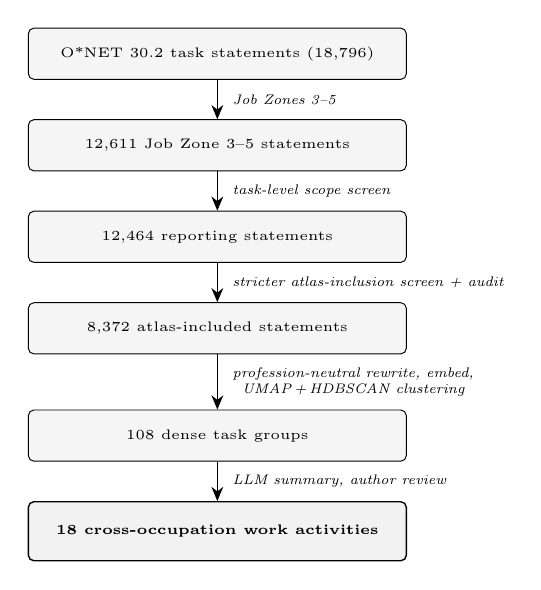
\begin{tikzpicture}[
  font=\tiny,
  every node/.style={align=center},
  data/.style={
    draw, rounded corners=2pt, fill=gray!8,
    inner sep=3pt, minimum height=6.5mm, minimum width=48mm,
    line width=0.35pt
  },
  final/.style={
    draw, rounded corners=2pt, fill=gray!10,
    inner sep=3pt, minimum height=7.5mm, minimum width=48mm,
    line width=0.5pt, font=\tiny\bfseries
  },
  arr/.style={-{Stealth[length=1.8mm,width=1.5mm]}, line width=0.45pt},
  lbl/.style={right=2pt, font=\tiny\itshape, anchor=west}
]
\node[data] (raw) {O{*}NET~30.2 task statements (18{,}796)};
\node[data, below=5mm of raw] (jobzone) {12{,}611 Job Zone 3--5 statements};
\node[data, below=5mm of jobzone] (screened) {12{,}464 reporting statements};
\node[data, below=5mm of screened] (retained) {8{,}372 atlas-included statements};
\node[data, below=7mm of retained] (groups) {108 dense task groups};
\node[final, below=5mm of groups] (ops) {18 cross-occupation work activities};

\draw[arr] (raw) -- node[lbl]{Job Zones 3--5} (jobzone);
\draw[arr] (jobzone) -- node[lbl]{task-level scope screen} (screened);
\draw[arr] (screened) -- node[lbl]{stricter atlas-inclusion screen + audit} (retained);
\draw[arr] (retained) -- node[lbl]{profession-neutral rewrite, embed,\\UMAP\,+\,HDBSCAN clustering} (groups);
\draw[arr] (groups) -- node[lbl]{LLM summary, author review} (ops);
\end{tikzpicture}%
}
\end{minipage}\hfill
\begin{minipage}[t]{0.60\linewidth}
\vspace{0pt}
\centering
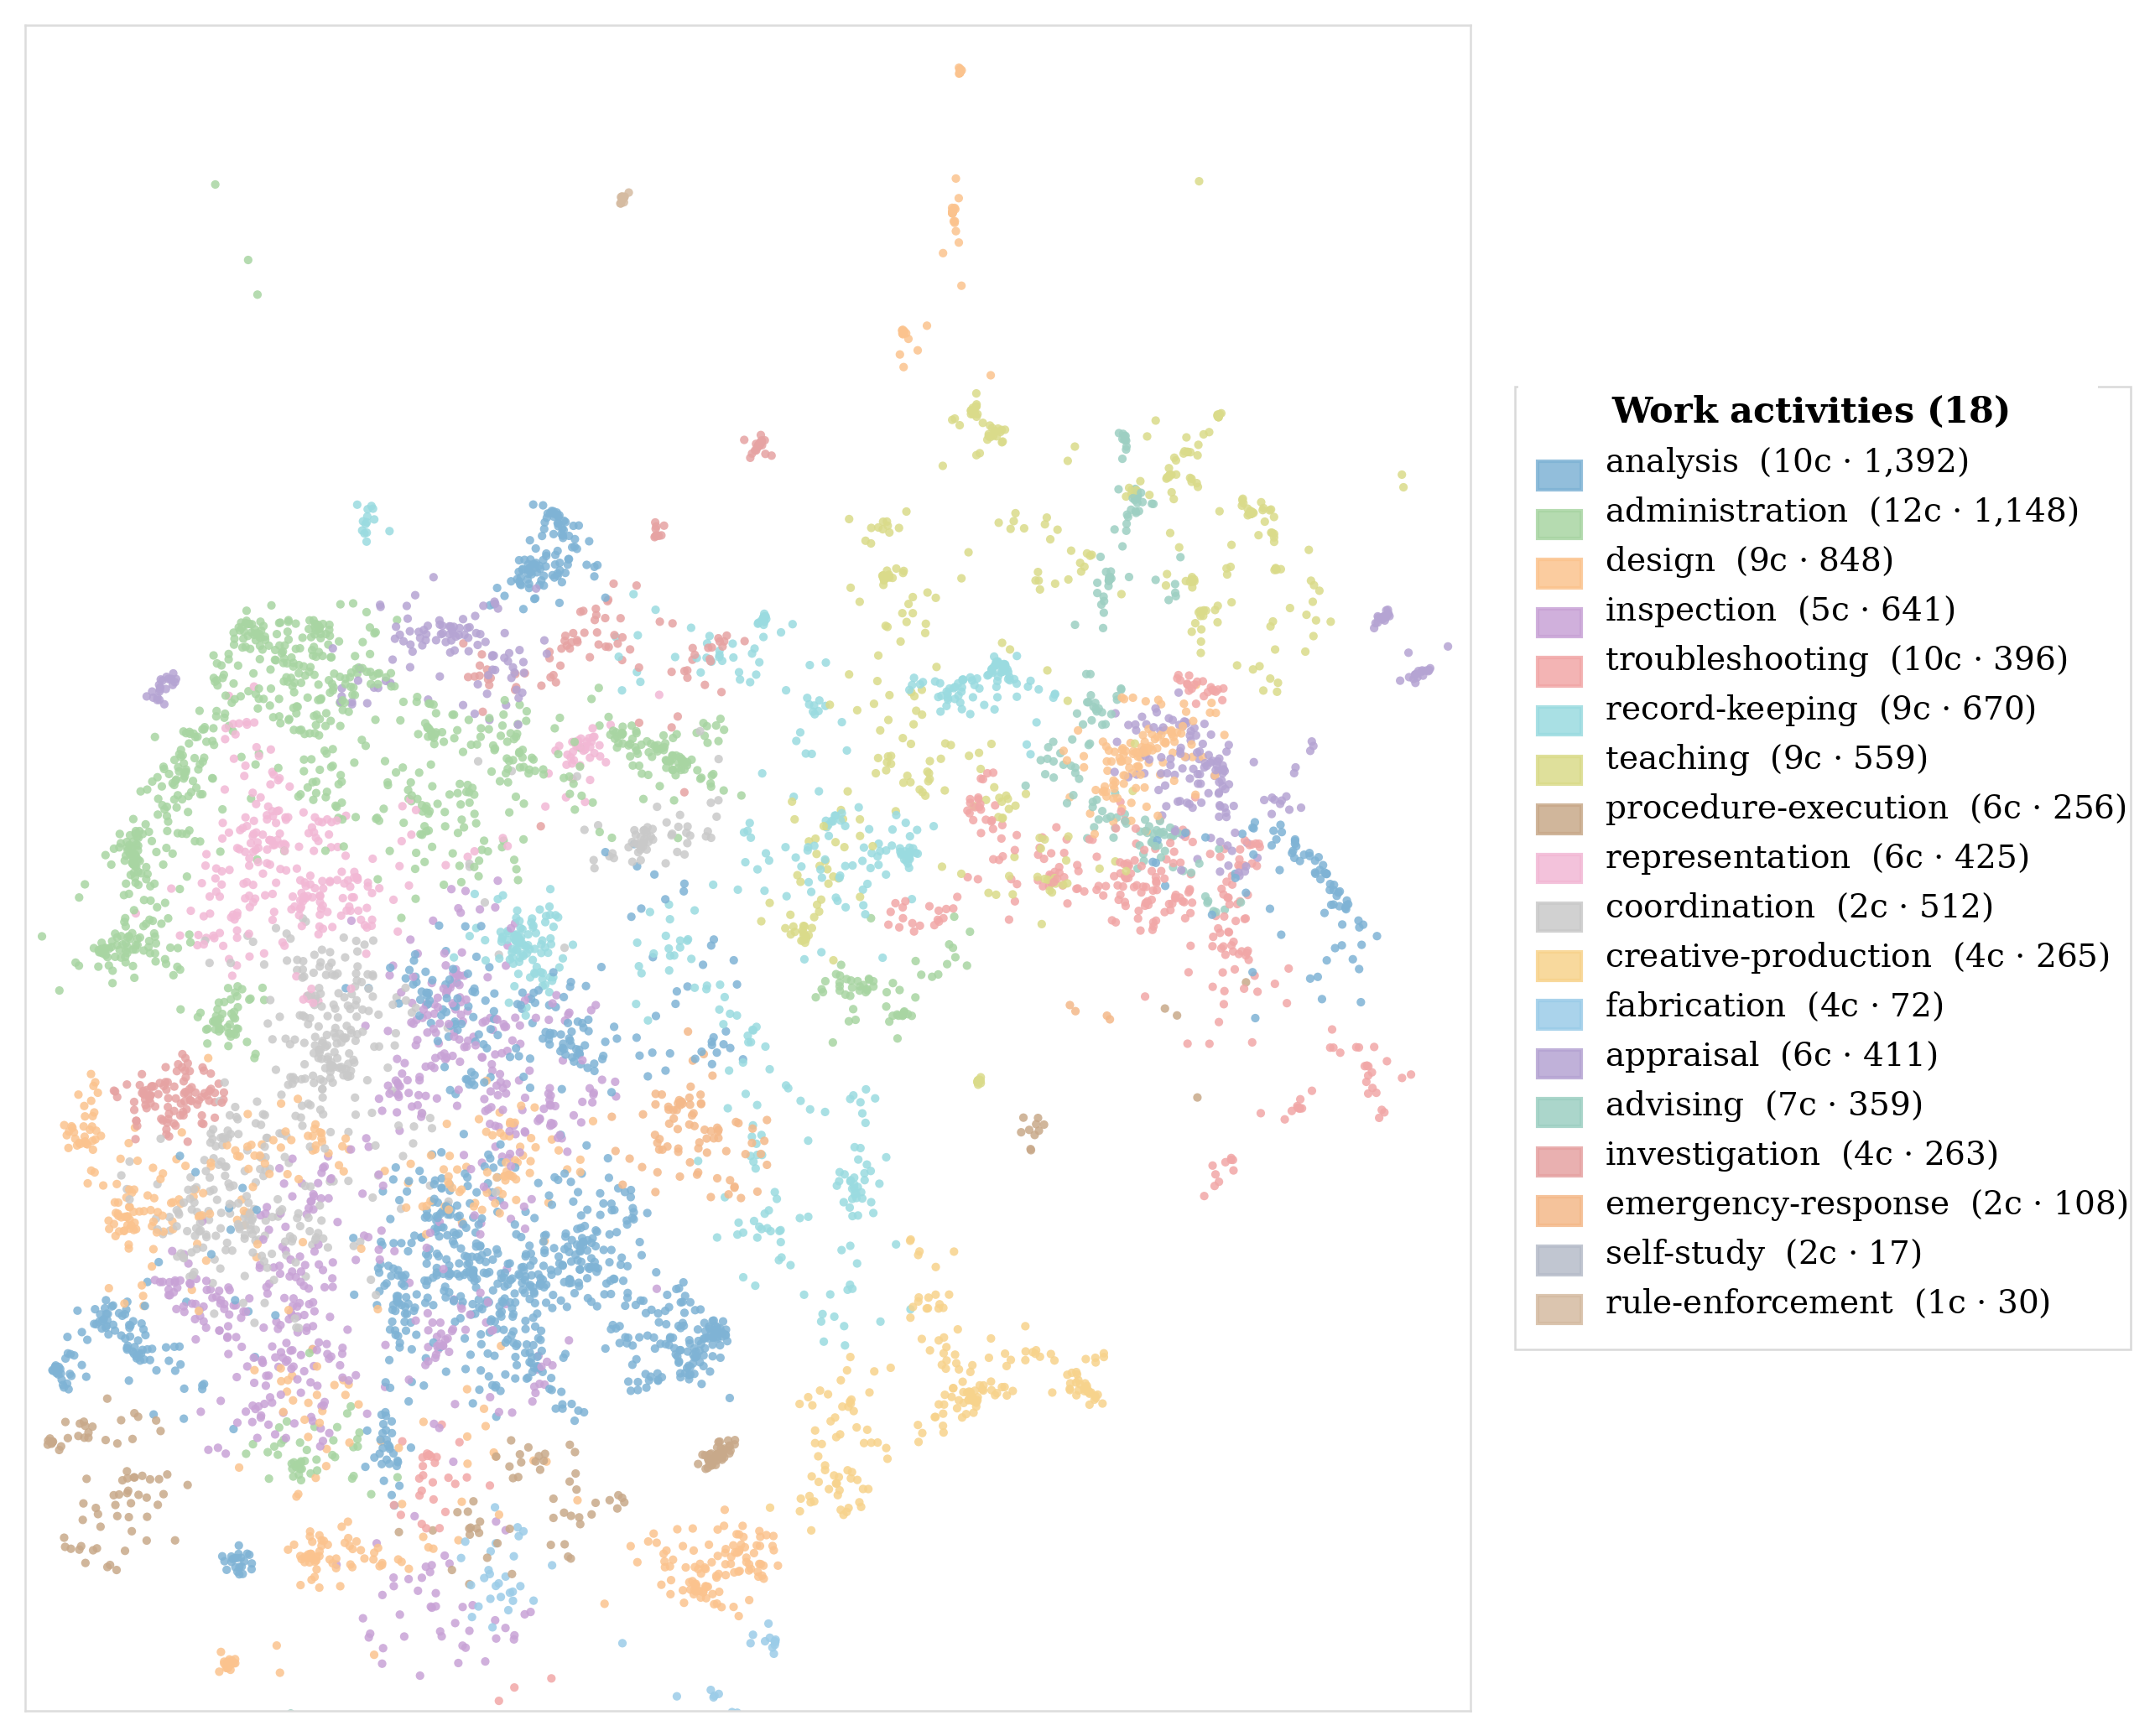
\includegraphics[width=\linewidth]{operation_atlas.png}
\end{minipage}

\par\vspace{2pt}
\begin{minipage}[t]{0.37\linewidth}
\centering\hspace*{8pt}\small\raisebox{-2pt}{(a) Construction pipeline}
\end{minipage}\hfill
\begin{minipage}[t]{0.60\linewidth}
\centering\small (b) Work-activity atlas
\end{minipage}
\caption{Construction and resulting atlas of the 18-work-activity inventory. Panel (a) separates the reporting corpus from the stricter atlas subset. Panel (b) shows the atlas used to inspect the work-activity grouping.}
\label{fig:inventory}
\end{figure}
\FloatBarrier

Table~\ref{tab:ops} reports the 18 work activities in the 12{,}464-task reporting corpus. NLP and agent benchmarks commonly report component tasks, task environments, or end-state success \citep{wang2024survey}; the activity field records the larger unit of work those components represent. An activity can be implemented through smaller benchmark tasks while retaining broader requirements for the transformation performed and the product left for review or use. A domain such as software engineering, healthcare, or office work can map to several activities, and each activity can be operationalized through smaller benchmark tasks. The benchmark report should state how those tasks represent the target activity and which parts remain outside the evaluation.

\begin{table}[!ht]
\caption{The 18 cross-occupation work activities derived from O{*}NET task statements. Counts are final activity assignments across the 12{,}464-task reporting corpus; the atlas subset contains 8{,}372 statements, so reporting and atlas counts differ by activity. The counts describe the reporting vocabulary and carry no labor-market weighting or AI deployment estimate. Occupations/settings and benchmark proxies are illustrative.}
\label{tab:ops}
\centering
\scriptsize
\setlength{\tabcolsep}{3pt}
\renewcommand{\arraystretch}{1.08}
\begin{tabularx}{\linewidth}{
@{}
>{\ttfamily\arraybackslash}p{0.16\linewidth}
>{\centering\arraybackslash}p{0.055\linewidth}
>{\raggedright\arraybackslash}p{0.32\linewidth}
>{\raggedright\arraybackslash}p{0.2\linewidth}
>{\raggedright\arraybackslash}X
@{}}
\toprule
\textbf{\normalfont Work activity} &
\textbf{\normalfont Tasks} &
\textbf{\normalfont Definition} &
\textbf{\normalfont Example settings} &
\textbf{\normalfont Common proxies} \\
\midrule
analysis &
1{,}732 &
Synthesize evidence into a supported finding or interpretation. &
Research; finance. &
Retrieval; summarization. \\
administration &
1{,}517 &
Plan, allocate, or maintain organizational resources or processes. &
Program management; operations. &
Form filling; state tracking. \\
design &
992 &
Specify a system, plan, artifact, or service to satisfy a goal. &
Product design; architecture. &
Plan generation; specification writing. \\
inspection &
963 &
Check a current state against rules, standards, or specifications. &
Compliance; safety review. &
Classification; checklist scoring. \\
troubleshooting &
902 &
Diagnose a problem and apply or recommend a remedy. &
IT support; software debugging. &
Log analysis; state repair. \\
record-keeping &
882 &
Create, update, store, or retrieve canonical organizational records. &
Clinical records; case files. &
Extraction; database update. \\
teaching &
814 &
Support a learner in acquiring knowledge or skill. &
Tutoring; professional training. &
Explanation; feedback generation. \\
procedure-execution &
735 &
Carry out a prescribed procedure according to a standard. &
Laboratory workflow; service procedure. &
Policy following; checklist execution. \\
representation &
615 &
Speak or act on behalf of an organization, client, or role. &
Client communication; advocacy. &
Role-play dialogue; policy-constrained response. \\
coordination &
603 &
Align actors, constraints, dependencies, or timing around shared work. &
Care coordination; logistics. &
Scheduling; task routing. \\
creative-production &
543 &
Produce an original creative, media, or communicative artifact to a brief. &
Marketing; media production. &
Copywriting; slide generation. \\
fabrication &
505 &
Plan or supervise the production, installation, or maintenance of a tangible asset from a work specification. &
Construction planning; equipment setup. &
Instruction generation; plan checking. \\
appraisal &
453 &
Assess, grade, value, or judge an artifact or case against a standard. &
Peer review; claims review. &
Rubric scoring; preference judgment. \\
advising &
403 &
Tailor a recommendation to a specific person, client, or case. &
Clinical advice; financial advice. &
Chat response; recommendation generation. \\
investigation &
377 &
Reconstruct an event, condition, or pattern from evidence. &
Fraud analysis; epidemiology. &
Timeline reconstruction; evidence retrieval. \\
emergency-response &
212 &
Stabilize or triage an acute incident under time pressure. &
Clinical triage; incident response. &
Triage classification; escalation decision. \\
self-study &
186 &
Maintain or update one's working competency through learning. &
Certification; continuing education. &
Learning plan; self-assessment. \\
rule-enforcement &
30 &
Apply or uphold behavioral or procedural rules in a setting. &
Conduct review; safety enforcement. &
Violation classification; escalation. \\
\bottomrule
\end{tabularx}
\end{table}

\subsection{Tested setting}
\label{sec:tested-setting}

Tested setting specifies the conditions in which the work activity is evaluated. A benchmark defines the materials, tools, role, and workflow state under which the task is completed, and these choices determine the evidence its result provides. Selected sources fix evidence selection in advance; a specified output form fixes product selection. These choices belong in the tested-setting description, together with whether the setting is itself the target or a simplified representation of a broader class of work settings.

\textsc{SWE-bench}, built from real GitHub issues \citep{jimenez2024swebench}, illustrates this distinction. The benchmark tests issue resolution under a repository snapshot, issue description, available files, and test suite. Requirement clarification, code review, and deployment sit outside that episode. Within the tested-setting field, the report should specify the materials available to the system and their status \citep{suchman1987plans,carlile2002pragmatic}. It should also record the tools and persistent states available for search, editing, or application use \citep{zhou2023webarena,xie2024osworld,drouin2024workarena}, the system's role and scope \citep{abbott1988system,freidson2001professionalism}, and the workflow state and dependencies at the start of the episode \citep{carlile2004transferring,malone1994coordination}.

The execution environment specifies which services, files, tools, credentials, and states exist. The tested setting adds which materials are authoritative, what role and authority the agent has, and which workflow stage the episode represents. A benchmark may intentionally evaluate one workflow stage, use cleaned source materials, restrict tools, or prescribe the output form; reporting these choices fixes the scope of the resulting claim.

\subsection{Required work product}
\label{sec:score-work-product}

Required work product defines what the activity should leave in the tested setting. The work product is the artifact or state the system is supposed to leave after completing the activity, such as a final response, revised document, database update, evidence trace, or handoff note. For prospective benchmark design, the intended work claim and receiving workflow define this product. For retrospective analysis, the benchmark's stated claim, task specification, and provided workflow are the primary evidence. When the benchmark itself invokes a broader occupational or workflow claim, additional product requirements can be inferred from that claim and are labeled as analytic inferences. A local task claim uses the object specified by the task as its required work product. A benchmark that evaluates source-grounded document revision should therefore define the revised artifact a reviewer would receive and the parts that must remain traceable and reviewable.

\subsection{Evaluated result}
\label{sec:scored-object}

Evaluated result records what the benchmark actually checks.
The evaluation design should state which parts of the required work product are checked by the metric, tests, or rubric.
A metric, test suite, or rubric provides evidence only for the properties it checks \citep{messick1989validity,kane2013validating}.
If the benchmark evaluates only a final answer, chat response, rewritten paragraph, or simulator success state, other parts of the work product remain untested.
Execution depth and evaluated result are separate choices: multi-step browsing or tool use can still terminate in a short evaluated answer.

In the document-revision example, evaluating only a rewritten paragraph can show that the system produced revised text, but it gives limited information about the full revision artifact.
Artifact-level evaluation would also check which locations were changed, whether source-supported content was preserved, whether unsupported or outdated content was corrected, whether citations, comments, or version structure remain traceable, and whether a reviewer can see the basis for the change.
Fluency and local textual improvement define a more limited target than the full source-grounded revision artifact.

Rubric design follows from the required work product. The work-product analysis determines what object ought to exist; the rubric, tests, or metric determine which properties of that object are checked.
When a benchmark aims to evaluate a broader work product, it should check whether the required materials were used, whether the system stayed within the assigned role, scope, and workflow state, and whether the resulting product preserves what a downstream actor or system needs for review or continuation.
Situated-action work motivates attention to source materials and local constraints \citep{suchman1987plans}, while knowledge-transfer work motivates attention to boundary crossing and downstream use \citep{carlile2002pragmatic,carlile2004transferring}.
General criteria such as helpfulness, clarity, or correctness can still be useful. A single aggregate judgment can combine unsupported evidence use, role violations, and missing handoff information with content quality.
When a rubric is used, the benchmark report should explain how each criterion follows from the expected work product and how the grader applies it. The four fields define the work-facing scope of a benchmark. They can guide task, setting, product, and evaluation design prospectively, or describe what an existing benchmark represents, evaluates, and leaves untested retrospectively. Figure~\ref{fig:officeqa-claim} illustrates how changing the intended work product changes what must be included in the evaluation.

\begin{figure}[!ht]
\centering
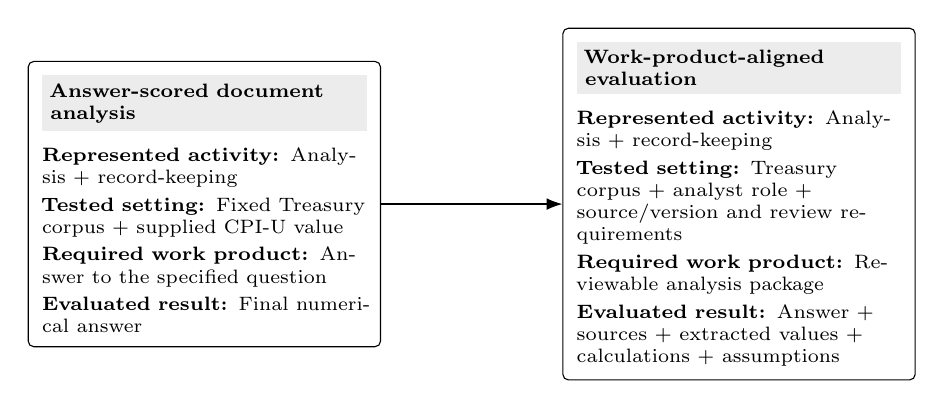
\begin{tikzpicture}[
  font=\scriptsize,
  card/.style={draw, rounded corners=2pt, align=left, inner sep=5pt, text width=0.34\linewidth},
  head/.style={fill=gray!12, draw=none, rounded corners=2pt, minimum width=0.32\linewidth, inner xsep=5pt, inner ysep=3pt, font=\bfseries\scriptsize, anchor=north west},
  arr/.style={-{Latex[length=2mm]}, line width=0.45pt}
]
\node[card] (qa) at (-0.28\linewidth,0) {
\colorbox{gray!15}{\parbox{\dimexpr\linewidth-2\fboxsep\relax}{\raggedright\bfseries Answer-scored document analysis}}\\[5pt]
\textbf{Represented activity:} Analysis + record-keeping\\[2pt]
\textbf{Tested setting:} Fixed Treasury corpus + supplied CPI-U value\\[2pt]
\textbf{Required work product:} Answer to the specified question\\[2pt]
\textbf{Evaluated result:} Final numerical answer};
\node[card] (broad) at (0.28\linewidth,0) {
\colorbox{gray!15}{\parbox{\dimexpr\linewidth-2\fboxsep\relax}{\raggedright\bfseries Work-product-aligned evaluation}}\\[5pt]
\textbf{Represented activity:} Analysis + record-keeping\\[2pt]
\textbf{Tested setting:} Treasury corpus + analyst role + source/version and review requirements\\[2pt]
\textbf{Required work product:} Reviewable analysis package\\[2pt]
\textbf{Evaluated result:} Answer + sources + extracted values + calculations + assumptions};
\draw[arr] (qa.east) -- (broad.west);
\end{tikzpicture}
\caption{Same represented activity, different work-product requirements and evaluation targets. The left panel shows an answer-scored document-analysis task of the form examined in \textsc{OfficeQA Pro}. When the intended product is a reviewable analyst deliverable, source/version information, extracted values, calculations, and assumptions also enter the evaluation.}
\label{fig:officeqa-claim}
\end{figure}

\section{Benchmark Case Analyses Through the Work-Centered Representation}
\label{sec:whybench}

This section applies the work-centered representation in Section~\ref{sec:guidelines} to three released benchmark cases.\footnote{Cases were selected to illustrate three scoring designs: expert-graded occupational deliverables, answer-scored grounded document analysis, and executable software-state changes.} We use one released instance per benchmark as a case-level demonstration. Benchmark-level coverage would require a stratified task sample within each suite and independent field assignment by a second coder. For each case, we populate the four fields and identify the boundary of the evaluated result.

\begin{table*}[!ht]
\caption{The four fields applied to the three released cases. The table reports the case-level interpretation used in the analyses below.}
\label{tab:case-comparison}
\centering
\footnotesize
\setlength{\tabcolsep}{4pt}
\renewcommand{\arraystretch}{1.12}
\begin{tabularx}{\textwidth}{@{}p{0.14\textwidth}X X X@{}}
\toprule
\textbf{Field} & \textbf{\textsc{GDPval}} & \textbf{\textsc{OfficeQA Pro}} & \textbf{\textsc{APEX-SWE}} \\
\midrule
Represented activity & \emph{Inspection} + \emph{design}. & \emph{Record-keeping} + \emph{analysis}. & \emph{Procedure-execution} + \emph{record-keeping}; troubleshooting enters if execution fails. \\
Tested setting & Federal grants-management role, fixed reference materials, task context, and required artifact. & Fixed Treasury Bulletin corpus, supplied CPI-U value, and closed numerical question. & Local \texttt{users.csv}, credentials, service documentation, LocalStack state, executable tests, and rubric. \\
Required work product & Federal Applicant Risk Assessment Tool for the specified grant-review task. & Numerical answer to the specified question. & Working Python script plus the required S3 object and state change. \\
Evaluated result & Submitted compliance artifact under head-to-head expert comparison. & Final number under exact-match or numerical-tolerance scoring. & Execution, S3 path, schema, and nonempty output; row-level correspondence with the source file is not checked. \\
\bottomrule
\end{tabularx}
\end{table*}

\textbf{\textsc{GDPval}} is introduced as a benchmark for evaluating model capabilities on real-world, economically valuable knowledge-work tasks, drawn from 44 occupations and 9 sectors, with an open gold subset of 5 cases per occupation. The benchmark provides task context and reference files, asks for deliverables such as documents, slides, and spreadsheets, and scores outputs through head-to-head expert comparison between the model deliverable and a human expert deliverable \citep{gdpval2025}. In a released compliance case (task id \texttt{36d567ba-e205-4313-9756-931c6e4691fe}), the model is placed in a federal grants management role and tasked with creating a Federal Applicant Risk Assessment Tool for grant review. The represented activities are primarily \emph{inspection} and \emph{design}. \emph{Record-keeping} enters through the tool's later use in review, while the released task itself ends at the submitted artifact. The tested setting specifies the role, reference materials, task context, and deliverable form. The evaluated result is the compliance artifact compared with a human expert artifact.

GDPval makes the task proxy explicit: a self-contained digital deliverable represents part of occupational work. The setting focuses on computer-based work and fixes task discovery in advance. The evaluation ends at deliverable quality; grant-review workflow linkage, approval records, filing actions, revision history, and audit trail lie outside the released case. The five-case public subset per occupation also leaves occupation-level coverage dependent on additional task-to-activity sampling.

\textbf{\textsc{OfficeQA Pro}} is introduced as a benchmark for grounded, multi-document reasoning over a large corpus of U.S. Treasury Bulletins. Its tasks require document parsing, retrieval, and analytical reasoning across text and tabular data, and the Pro split uses hard questions with verifiable answers \citep{opsahlong2026officeqapro}. The national-defense expenditure case (task id \texttt{UID0005}) asks the model to use reported monthly values from 1953 and 1940, incorporate an external annual-average CPI-U value, apply inflation correction, and round the result. Under the work-centered representation, the case represents \emph{record-keeping} and \emph{analysis}: the model must locate the correct Treasury Bulletin records and combine the retrieved values with the external value in a specified calculation. The tested setting is a fixed document corpus with a closed analytical question, and the evaluated result is the final numerical answer under exact-match or numerical-tolerance scoring. Closed questions support reproducible numerical scoring. The evaluation ends at the final value. A reviewable analyst product would additionally contain the cited source and version, extracted values and units, intermediate calculations, and relevant assumptions or conflicts, with those components included in the evaluation.

\textbf{\textsc{APEX-SWE}} is introduced as a benchmark for economically valuable software-engineering tasks. Integration tasks require end-to-end systems across cloud primitives, business applications, and infrastructure services, while Observability tasks require debugging production-style failures using telemetry and unstructured context. Released tasks provide containerized environments, issue context, service documentation, connection information, pytest tests, and rubric files \citep{kottamasu2026apex}. In the \texttt{1-aws-s3-snapshots} case, the model must create a Python script that uploads a local \texttt{users.csv} file to a date-based LocalStack S3 path. The represented activities are primarily \emph{procedure-execution} and \emph{record-keeping}, with \emph{troubleshooting} entering when execution failures must be resolved inside the benchmark environment. The tested setting supplies local data, credentials, service state, documentation, and executable tests. The required work product is a working script plus the specified S3 state change. Tests check execution, path, schema, and nonempty output. The released reference solution reads the local \texttt{users.csv} file as specified, while the tests leave row-level correspondence between the source file and uploaded object unchecked \citep{mercor2026apexs3}.

The APEX-SWE case therefore checks local ticket completion and endpoint state more strongly than source-to-state fidelity. Production deployment, access-control review, and rollback occur beyond the released integration episode. A source-fidelity claim would require a check that links the uploaded rows to the specified source file. Across the three cases, the same four fields expose different boundaries. \textsc{GDPval} ends at deliverable quality before downstream grant-workflow linkage; \textsc{OfficeQA Pro} checks the final numerical answer without a reviewable source-and-calculation record; \textsc{APEX-SWE} checks executable endpoint state more strongly than source-to-state fidelity.

\paragraph{Artifacts and reproducibility.}
The supplementary archive includes machine-readable definitions for the 18 activities and the validation summary in Appendix~\ref{app:taxonomy}. The full 12{,}464-task O{*}NET assignments and item-level ESCO mappings are stored as derived files and will be released with the final archival version. Appendix~\ref{app:taxonomy} describes the inventory construction and validation; Appendix~\ref{app:esco} describes the ESCO mapping and aggregate results.

\section{Discussion}
\label{sec:altviews}

When a benchmark score is interpreted as evidence about work, the claim should be stated at the same grain as the evidence: the activity represented, the conditions tested, the product expected, and the result checked. Direct workplace studies can answer a specified local question without an intermediate benchmark. Field and experimental studies can measure productivity, quality, and other outcomes in a defined population and workflow \citep{dellacqua2023jagged,brynjolfsson2023genai}. When the population, workflow, outcome, and decision match the intended use, that study directly supports the local conclusion. Generalization to another organization, role, interface, task distribution, or outcome requires additional evidence. Public benchmarks serve a different function by providing repeatable pre-deployment comparisons across systems. Reporting activity, setting, product, and evaluated result makes the boundary of that evidence visible.

Representative work samples and predictive proxies also support different claims. A benchmark sampled from an explicit job or workflow frame and scored on the products or outcomes used in practice can assess that sampled domain directly \citep{roth2005worksample}. Simpler capability measures can support model ranking or forecasting when their predictive relationship is established in the target domain \citep{ruan2024observational}. Portfolio-level mappings can describe where evaluation effort is concentrated across occupations and skills \citep{wang2026realwork}. Work claims that extend beyond those objectives require the role, workflow state, work product, and evaluated result to be stated explicitly. Component evaluations are self-contained when the claim is component-level. Retrieval and embedding benchmarks isolate specific behaviors and make failures easier to locate \citep{thakur2021beir,muennighoff2022mteb}. A broader claim about analysis, advising, coordination, or record-keeping also depends on how that component is used in the tested setting and what product the workflow requires.

The O{*}NET inventory supplies one vocabulary for the represented-activity field. Work practices vary across institutions and over time \citep{suchman1987plans,kellogg2020algorithms}, while O{*}NET task statements describe occupational work at a more general level and inherit the limits of an occupational information system \citep{handel2016onet,onet2024tasks}. The inventory can therefore be revised or replaced as stronger workflow evidence becomes available. Its role here is to give benchmark reports a shared middle-level vocabulary between component tasks and occupations.

Future benchmark development can move more of the required work product into evaluation. Coding-agent benchmarks already score repository state, patches, and executable tests \citep{jimenez2024swebench,kottamasu2026apex}. Web, desktop, and enterprise-agent benchmarks expose different materials, tools, and persistent states \citep{zhou2023webarena,xie2024osworld,drouin2024workarena}. For document, clinical, or research work, the same design logic begins with the represented activity and tested setting, specifies the product another actor or system receives, and checks the parts of that product needed for the intended claim. Knowledge-work benchmark results can enter decisions about automation, procurement, and staffing. The four fields keep those interpretations tied to the activities, settings, products, and evaluated results actually tested. Occupation-level workforce claims require evidence at the occupation and workplace level.

The activity inventory also needs broader validation. Comparisons with other occupational ontologies, observed workflows, and workplace-use traces can test whether the current labels remain useful beyond O{*}NET \citep{esco2022v111,handa2025economic}. The open-label interpretability check in Appendix~\ref{app:taxonomy} used two validators over 18 blinded cards; a larger, independently recruited panel scoring more task examples per activity would show whether observed confusions, such as \emph{procedure-execution} being read as navigation, persist across examples. The case analyses can be extended through stratified, multi-instance samples within each benchmark and independent field coding with adjudicated disagreements. A separate study can test use of the representation itself by comparing benchmark-design choices with and without the four-field report. These two extensions address benchmark coverage and practical utility, respectively.

\section{Conclusion}
\label{sec:conclusion}

AI-agent benchmarks increasingly target workplace-facing tasks. Knowledge work varies in the activity performed, the setting in which it occurs, and the product that should remain after completion.
This paper develops a work-centered benchmark representation with four fields: represented activity, tested setting, required work product, and evaluated result.
The benchmark case analyses illustrate how occupational deliverables, grounded answers, and executable state changes capture different parts of work within the same representation.
Benchmark design can begin with the work activity and tested setting, define the work product the activity should leave, and then choose an evaluation target that checks the relevant parts of that product.
Reporting these elements makes the scope of a work claim explicit when agents are tested in work-shaped settings.

\newpage
\renewcommand{\bibfont}{\normalsize}
\bibliographystyle{plainnat}
\bibliography{references}

\newpage
\appendix
\renewcommand{\thefigure}{\Alph{section}.\arabic{figure}}
\renewcommand{\thetable}{\Alph{section}.\arabic{table}}
\makeatletter
\@addtoreset{figure}{section}
\@addtoreset{table}{section}
\makeatother
\setcounter{figure}{0}
\setcounter{table}{0}

\section{Inventory construction details}
\label{app:taxonomy}

\paragraph{Corpus.}
This appendix documents how the 18-work-activity inventory used in Section~\ref{sec:define-work} is built from O{*}NET task text \citep{onet2024tasks}. Figure~\ref{fig:inventory}(a) diagrams the full pipeline, including the embedding, UMAP, and HDBSCAN clustering stage that yields 108 dense task groups before author consolidation \citep{mcinnes2018umap,campello2013density}. Starting from 18{,}796 O{*}NET~30.2 task statements, we restrict the candidate occupational scope to occupations assigned Job Zones~3--5, yielding 12{,}611 statements \citep{onet2024tasks}. The Job Zone restriction defines the broad occupational scope. GPT-5.5-assisted screening with author adjudication removes 147 residual statements whose primary content is direct manual, performative, or routine clerical work, leaving a reporting corpus of 12{,}464 task statements. Each retained row carries the O{*}NET-SOC code, occupation title, task identifier, cleaned task text, importance and relevance scores, and Job Zone.

\paragraph{Screens.}
The screening procedure uses iterative GPT-5.5 classification with author adjudication. The exclusion categories are developed through three independent 100-task samples drawn without replacement from the candidate corpus; each sample is adjudicated against a growing list of candidate exclusion categories until the list stabilizes at twelve categories. The screen targets execution-level manual, performative, and routine-clerical work; planning, specification, supervision, and review of tangible work remain eligible when the task product is cognitive or documentary.
A stricter atlas-inclusion screen is then applied to the 12{,}464-task reporting corpus. It initially excludes 4{,}126 statements; author audit re-includes 34 availability-scheduling statements, yielding 8{,}372 statements for profession-neutral rewriting, embedding, clustering, and consolidation. The final 18 work-activity labels are applied to the 12{,}464-task reporting corpus for Table~\ref{tab:ops}, while the atlas visualizes the stricter 8{,}372-task subset.

\paragraph{Embedding and clustering.}
Tasks are rewritten into profession-neutral work-activity phrases under a fixed prompt to remove domain vocabulary, then embedded with \texttt{text-embedding-3-small} into a $1{,}536$-dimensional space and $L_{2}$-normalized.
UMAP with 15 dimensions, 30 neighbors, cosine distance, minimum distance 0, and seed 42, followed by HDBSCAN with minimum cluster size 30, minimum samples 10, and excess-of-mass extraction, yields 108 clusters on the task-only geometry; 4{,}487 points marked as noise are soft-assigned for downstream review via membership vectors \citep{mcinnes2018umap,campello2013density}.

\paragraph{Consolidation.}
The authors review all 108 source clusters and merge or separate groups according to the transformation performed and the product left by the work. Four rounds of Claude Opus~4.7 summarization at temperature 0.1 propose domain-stripped cluster labels; human review determines the retained set. Rounds 1--3 produce 38, 39, and 16 top-level activities and are not retained. The fourth round produces 19 candidate activities, including separate \emph{inspection} and \emph{investigation} labels. Human review folds a 93-task clinical~/~surgical~/~nursing-support cluster into \emph{procedure-execution}, yielding the final 18 activities used in Figure~\ref{fig:inventory} and Table~\ref{tab:ops}.

\paragraph{Invariants.}
Every atlas cluster has exactly one top-level assignment, and every top-level work activity has $\geq\!1$ member cluster and several distinct occupation families in its cross-occupation example set. For reporting, the final labels are propagated to all 12{,}464 screened task statements, so Table~\ref{tab:ops} conserves the reporting corpus. The assignment step is uneven across activities: \emph{self-study} changes from 17 atlas tasks to 186 reporting assignments (10.9$\times$), \emph{fabrication} from 72 to 505 (7.0$\times$), and \emph{rule-enforcement} remains 30 to 30 (1.00$\times$). These ratios diagnose assignment-boundary breadth; the reporting counts carry no labor-market prevalence interpretation. ESCO assigns 128 of 5{,}730 mapped items (2.2\%) to \emph{rule-enforcement}, providing a separate frequency signal from another occupational ontology. Every work activity also carries explicit contrasts against adjacent activities. \emph{Self-study} refers to active maintenance or updating of working competency; attendance obligations alone fall outside this activity definition.

\paragraph{Validation.}
The frozen inventory is evaluated through semantic coherence, algorithm sensitivity, ESCO legibility, and two human interpretability checks. Two independent validators recover most activity labels without definitions and match all 18 after the definitions are shown (Table~\ref{tab:inventory-validation}). The same validation identifies weaker boundaries for \emph{procedure-execution} and \emph{record-keeping}.

\begin{table*}[!ht]
\caption{Five validation questions for the 18-work-activity reporting vocabulary, with the evidence, interpretation, and remaining limit for each check.}
\label{tab:inventory-validation}
\centering
\footnotesize
\setlength{\tabcolsep}{4pt}
\renewcommand{\arraystretch}{1.12}
\begin{tabularx}{\textwidth}{@{}p{0.14\textwidth}p{0.34\textwidth}p{0.23\textwidth}X@{}}
\toprule
\textbf{Question} & \textbf{Evidence and result} & \textbf{Interpretation} & \textbf{Limit} \\
\midrule
Internal coherence & Task-to-activity-centroid cosine similarity and blinded 1--5 human coherence ratings. Activity median similarity 0.538--0.911; weighted mean 0.581. Validator means 3.833 and 4.056; median 4 for both. & Tasks grouped under an activity have interpretable semantic concentration. & Partition uniqueness remains unresolved by this descriptive similarity check. \\
Algorithm sensitivity & KMeans at $k=40$ compared with HDBSCAN non-noise assignments. Adjusted Rand index 0.460; normalized mutual information 0.822. & A related broad organization appears under a different algorithm. & Seed sensitivity remains unmeasured; $k=40$ also represents a different granularity. \\
External ontology legibility & The frozen activity vocabulary is applied to independently developed ESCO v1.1.1 skills and checked against a nearest-neighbor permutation baseline. Of 5{,}826 scoped skills, 5{,}730 are mapped; all 18 activities receive assignments; 3{,}893 are high-confidence. Nearest-neighbor same-activity agreement is 45.15\% versus 8.52\% after label permutation. & The frozen vocabulary remains usable on ESCO and the assigned labels show non-random local structure in ESCO embedding space. & Task-classification accuracy and item-level mapping correctness remain unmeasured. \\
Open-label interpretability & Two independent validators review 18 blinded task cards in randomized order using open labels, coherence ratings, and outlier marking. Exact coherence agreement is 12/18; agreement within one point is 18/18; quadratic-weighted $\kappa=0.802$. Strict direct recovery is 15/18 and 16/18; direct-or-partial recovery is 17/18 for each validator; three joint outliers occur among 71 task examples. & Most activities can be independently recognized without seeing the definitions. & Two validators, manually selected cards, author-coded correspondence, and partial corpus annotation. \\
Definition recognition & Stage-2 matching is performed after definitions are revealed. Both validators match 18/18. & The definitions are legible and distinguishable after exposure. & This is a definition-legibility check; procedure-execution remained the weakest open-label abstraction. \\
\bottomrule
\end{tabularx}
\end{table*}

\section{External ontology check: ESCO}
\label{app:esco}

\paragraph{Source and scope.}
This appendix reports the ESCO legibility experiment: its scope, design, pipeline, per-work-activity mapping results and shares, and the cases where the O{*}NET and ESCO per-work-activity distributions diverge. The ESCO inputs are the v1.1.1 English CSV release \citep{esco2022v111}, ingesting the Skills pillar, the Occupations pillar with the ISCO groups table, and the occupation--skill relations.
The scope filter keeps rows whose skill type is skill or competence and retains only skills that are essential-linked to at least one occupation in ISCO-08 groups 1, 2, or 3, giving 5{,}826 items \citep{esco2022v111}.
A supplementary set of 1{,}977 knowledge-type items describes subject-matter domains and is excluded from the activity-focused primary analysis.

\paragraph{Design.}
O{*}NET remains the derivation dataset and the 18 labels are held frozen for the ESCO check. ESCO describes skills and competences, while O{*}NET task statements describe work performed, so the two sources are analyzed at their native units. The ESCO scope keeps skills or competences linked as essential to at least one ISCO-08 group 1--3 occupation \citep{ilo2012isco08}, corresponding to the O{*}NET Job Zones 3--5 occupational scope.
The resulting 5{,}826 items are assigned to one of the 18 work activities by \texttt{gpt-5.4-mini} using the frozen per-work-activity definition, input, output, and distinct-from fields, plus a ``none of the above'' option.
The signals we report are the mapping result under this rubric assignment, nearest-neighbor label consistency in the ESCO embedding space, and the per-work-activity distribution of ESCO items against the O{*}NET distribution in Table~\ref{tab:ops}.
The divergences localize the places where the inventory is most O{*}NET-shaped, and their direction is interpretable from how the two ontologies are built.

\paragraph{LLM assignment.}
\texttt{gpt-5.4-mini} is called once per item at temperature 0 with the 18 work-activity ids and their one-line definition, input, output, and up to three distinct-from clauses.
The prompt requires the model to return a work-activity id, a confidence rating of high, medium, or low, and a one-sentence rationale, and explicitly permits a ``none of the above'' label for items that do not describe a work activity.
Classification calls are cached so the pass is resumable.
Of the 5{,}826 scoped items, 3{,}893 return high confidence (66.8\%), 1{,}642 medium (28.2\%), and 291 low (5.0\%).
We additionally assess geometry-only label consistency using nearest-neighbor agreement in the 1{,}536-dimensional \texttt{text-embedding-3-small} cosine space; the permutation baseline shuffles the assigned work-activity labels before repeating the same calculation.
A supplementary centroid assignment, based on cosine similarity of each ESCO item to the $L_{2}$-normalized mean of O{*}NET task embeddings per work activity, is computed for cross-reference and excluded from the reported appendix numbers.

\paragraph{Mapping result.}
5{,}730 of the 5{,}826 ESCO items (98.3\%) are placed into one of the 18 work activities; 96 items (1.7\%) receive a ``none of the above'' label.
All 18 work activities receive ESCO items; 17 of 18 receive $\geq\!40$ items, with \emph{investigation} the single exception at 39.
The ``none of the above'' set mainly contains worker attributes and subject-matter labels, which fall outside the work-activity representation.
Under this rubric assignment, the frozen vocabulary covers most scoped ESCO items at the categorical level: no work activity is empty and only a small residue is assigned outside the inventory.
Where the two corpora diverge is in how they re-weight the 18 work activities, which we read next.

\paragraph{Where O{*}NET and ESCO diverge.}
Figure~\ref{fig:esco_share} and Table~\ref{tab:esco_mapping} give the per-work-activity shares in each corpus.
Every work activity is populated in both corpora. Their different source units produce substantial re-weighting across activities.
O{*}NET is a task inventory and places more weight on repeated task statements within occupations. ESCO is a skill and competence catalog and places more weight on transferable competences.
The divergence shows that the 18-work-activity vocabulary remains legible across a separate occupational ontology while its activity frequencies retain the imprint of the O{*}NET derivation source. The ESCO experiment measures legibility under corpus shift with the 18 labels held fixed.

\begin{figure}[!ht]
\centering
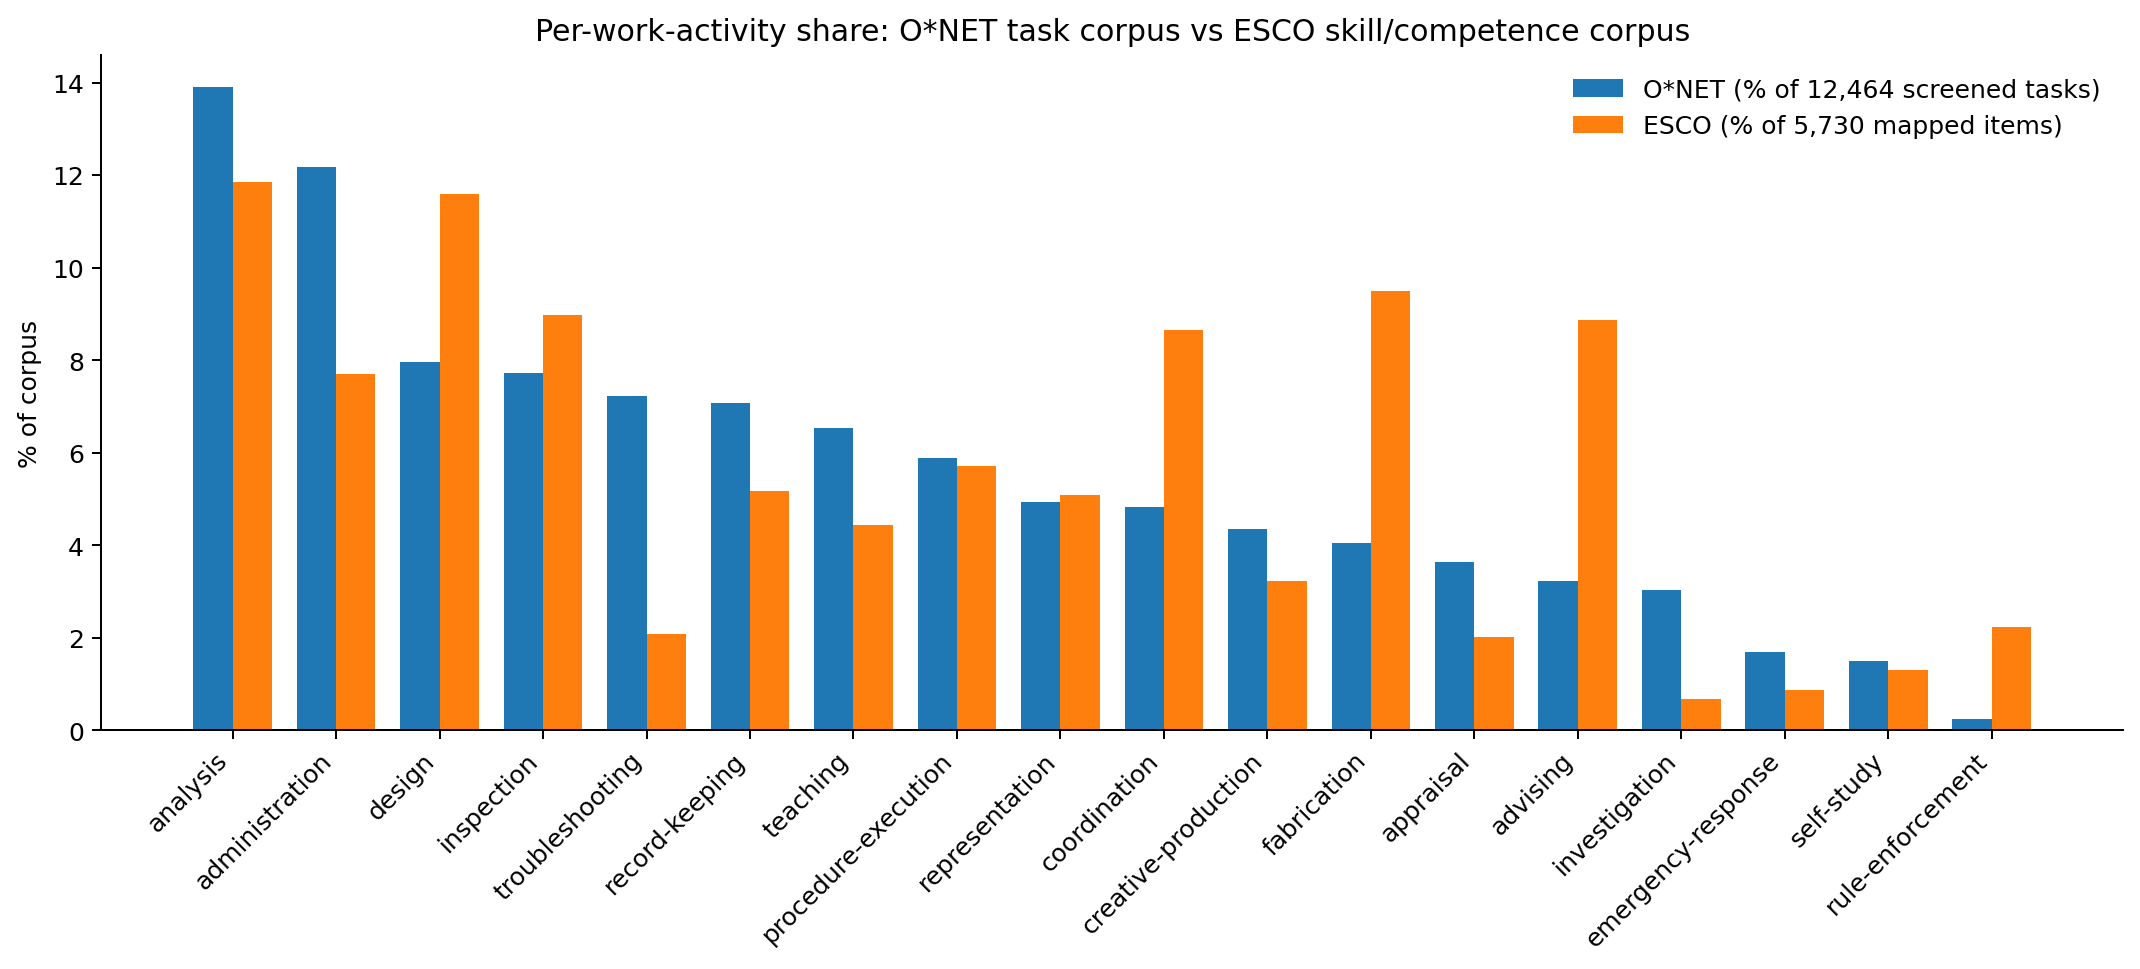
\includegraphics[width=0.98\linewidth]{esco_onet_op_share.png}
\caption{\textbf{Per-work-activity share in the O{*}NET task corpus
  (12{,}464 screened reporting tasks) versus the scoped ESCO
  skill/competence corpus (5{,}730 items mapped to a work activity).}
  Both corpora populate all 18 work activities. The two catalogs
  re-weight the work activities substantially: ESCO emphasizes
  \emph{advising}, \emph{fabrication}, and \emph{coordination} more than O{*}NET;
  O{*}NET emphasizes \emph{troubleshooting}, \emph{administration}, and
  \emph{record-keeping} more than ESCO. The direction of the divergence
  tracks the two ontologies' different source units
  (domain-bound tasks vs profession-abstract competences), as
  read in Appendix~\ref{app:esco}. Underlying counts are in
  Table~\ref{tab:esco_mapping}.}
\label{fig:esco_share}
\end{figure}

\begin{table}[!ht]
\caption{Per-work-activity shares in the O{*}NET task corpus versus the
  scoped ESCO skill/competence corpus. \textbf{O{*}NET $n$} is the
  task count from Table~\ref{tab:ops}. \textbf{ESCO $n$} is the number
  of scoped ESCO items assigned to the work activity by the LLM
  classifier. \textbf{$\Delta$} is ESCO percent minus
  O{*}NET percent in work-activity-share percentage points. Sorted by
  $\Delta$.}
\label{tab:esco_mapping}
\centering
\footnotesize
\begin{tabular}{lrrrrr}
\toprule
work activity & O{*}NET $n$ & O{*}NET \% & ESCO $n$ & ESCO \% & $\Delta$ (pp) \\
\midrule
\emph{troubleshooting}      &    902 &  7.2 & 120 &  2.1 & $-5.1$ \\
\emph{administration}       & 1{,}517 & 12.2 & 441 &  7.7 & $-4.5$ \\
\emph{investigation}        &    377 &  3.0 &  39 &  0.7 & $-2.3$ \\
\emph{teaching}             &    814 &  6.5 & 254 &  4.4 & $-2.1$ \\
\emph{analysis}             & 1{,}732 & 13.9 & 679 & 11.9 & $-2.0$ \\
\emph{record-keeping}      &    882 &  7.1 & 297 &  5.2 & $-1.9$ \\
\emph{appraisal}            &    453 &  3.6 & 116 &  2.0 & $-1.6$ \\
\emph{creative-production} &    543 &  4.4 & 185 &  3.2 & $-1.1$ \\
\emph{emergency-response}  &    212 &  1.7 &  50 &  0.9 & $-0.8$ \\
\emph{self-study}          &    186 &  1.5 &  75 &  1.3 & $-0.2$ \\
\emph{procedure-execution}  &    735 &  5.9 & 328 &  5.7 & $-0.2$ \\
\emph{representation}       &    615 &  4.9 & 292 &  5.1 & $+0.2$ \\
\emph{inspection}           &    963 &  7.7 & 514 &  9.0 & $+1.2$ \\
\emph{rule-enforcement}    &     30 &  0.2 & 128 &  2.2 & $+2.0$ \\
\emph{design}               &    992 &  8.0 & 664 & 11.6 & $+3.6$ \\
\emph{coordination}         &    603 &  4.8 & 496 &  8.7 & $+3.8$ \\
\emph{fabrication}          &    505 &  4.1 & 544 &  9.5 & $+5.4$ \\
\emph{advising}             &    403 &  3.2 & 508 &  8.9 & $+5.6$ \\
\midrule
\textbf{total}                & \textbf{12{,}464} & \textbf{100.0} & \textbf{5{,}730} & \textbf{100.0} & \\
\bottomrule
\end{tabular}
\end{table}
\FloatBarrier



\section{Design notes for each work activity}
\label{app:opslens}

Table~\ref{tab:opslens} translates the 18 work activities into benchmark-design notes.
The table applies the same four-field logic to each activity by pairing a plausible benchmark proxy with the work-product evidence relevant to that activity.

\begin{table}[!ht]
\caption{Design notes for applying the work-centered representation to each work activity.}
\label{tab:opslens}
\centering
\scriptsize
\begin{tabularx}{\linewidth}{lXX}
\toprule
work activity & plausible benchmark proxy & what the scored work product should show \\
\midrule
\emph{analysis} & Interpretive memo from heterogeneous evidence. & The product should preserve source support, assumptions, reasoning path, and a finding that a reviewer can inspect. \\
\emph{administration} & Multi-platform workflow task across records, approvals, or enterprise systems. & The product should show the updated state, the authority for the update, and the remaining handoff or approval step. \\
\emph{design} & Specification for a system, service, artifact, or process. & The product should be executable by a downstream actor and should state constraints, tradeoffs, and acceptance criteria. \\
\emph{inspection} & Review of an artifact against rules, standards, or clauses. & The product should cite the governing rule, identify the checked item, and separate conforming from nonconforming findings. \\
\emph{troubleshooting} & Diagnose-and-fix task in software, clinical, technical, or operational settings. & The product should include the diagnosis, the evidence for it, the fix or recommendation, and a check that the problem state changed. \\
\emph{record-keeping} & Retrieve, update, reconcile, or file a canonical record. & The product should preserve version, provenance, field-level changes, retention constraints, and retrieval path. \\
\emph{teaching} & Tutorial or feedback episode for a learner. & The product should show the learning goal, learner state, feedback given, and evidence that the learner can use the instruction. \\
\emph{procedure-execution} & Execute a prescribed procedure under a stated standard. & The product should show each required step, deviations, escalation decisions, and final procedural status. \\
\emph{representation} & Act or communicate on behalf of a person, organization, or role. & The product should show role authority, constraints, commitments made, and the external-facing record. \\
\emph{coordination} & Align actors, timing, dependencies, or handoffs across tools. & The product should show responsibilities, dependencies, unresolved blockers, and the next actor who receives the work. \\
\emph{creative-production} & Produce a media, design, or communication artifact from a brief. & The product should satisfy the brief, preserve required assets or constraints, and be deliverable in the requested format. \\
\emph{fabrication} & Plan or supervise tangible work from a specification. & The product should show the work plan, material or safety constraints, acceptance checks, and the limits of non-embodied evaluation. \\
\emph{appraisal} & Grade, value, review, or judge an artifact or case. & The product should state the standard used, the evidence inspected, the judgment, and reasons a second reviewer can audit. \\
\emph{advising} & Tailored recommendation for a person, client, or case. & The product should show case facts, options considered, scope limits, risk or uncertainty, and the action the recipient can take. \\
\emph{investigation} & Reconstruct an event, condition, or pattern from evidence. & The product should show evidence collection, source conflicts, timeline or causal reconstruction, and unresolved gaps. \\
\emph{emergency-response} & Time-pressured triage or incident response. & The product should show immediate risk assessment, escalation decision, action taken, time-sensitive constraints, and handoff. \\
\emph{self-study} & Maintain or update working competency through active learning or review. & The product should show learning need, materials used, competency update, and evidence of retained or usable knowledge. \\
\emph{rule-enforcement} & Apply behavioral or procedural rules in context. & The product should show the rule, observed conduct, contextual exception if any, decision, and appeal or escalation path. \\
\bottomrule
\end{tabularx}
\end{table}
\FloatBarrier

\end{document}
